
\chapter{Project schedule from Initial Document}
\label{app:project_schedule}

    You can see the project schedule we included in the Initial document in Appendix \ref{app:project_schedule} on page \pageref{app:project_schedule}. We have distinguished categories of tasks in the schedule through colour coding. Green represents tasks that are directly related to the completion of the project, whether it be research, design, implementation, or testing. Blue bars represent tasks related to the deliverables required by the university besides the Android Image. Grey tasks are periods of time reserved to focus on other courseworks or on exams. Finally, orange tasks are for the completion of secondary project objectives.
    
    \begin{landscape}
    \begin{figure}[H]
    	% [H] means put the figure HERE, directly when you input this code.
    	\centering
    	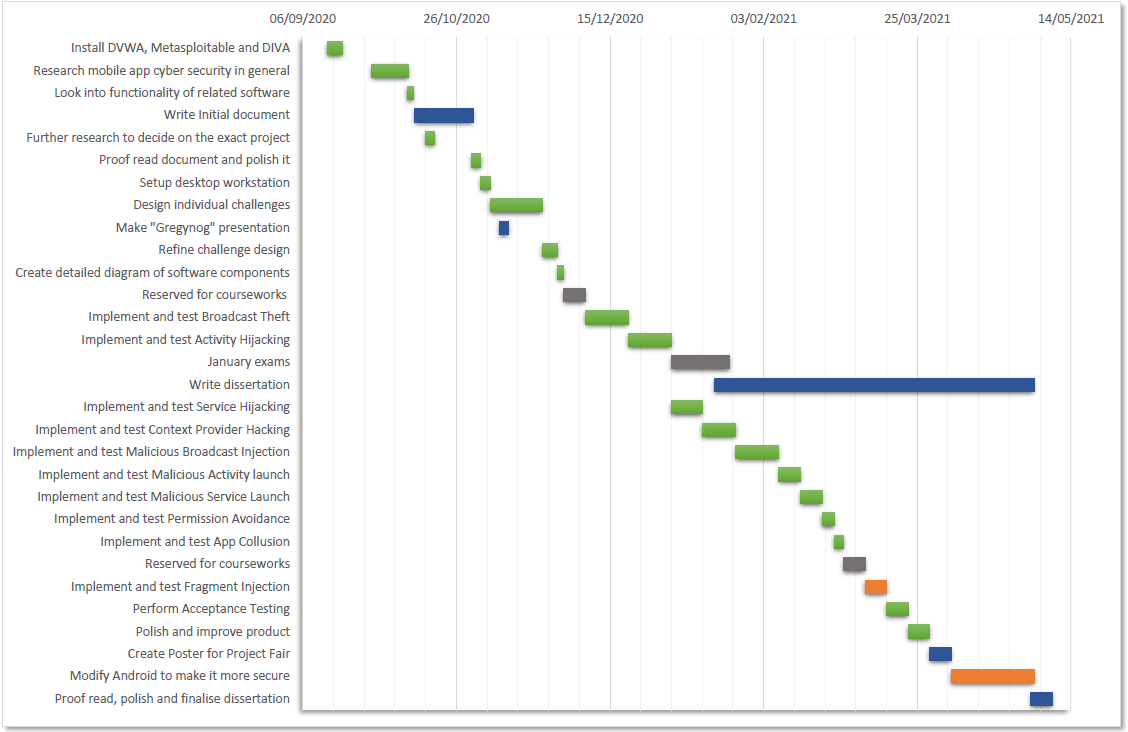
\includegraphics[width=1\linewidth]{./graphics/schedule.PNG}
    	
    	% Caption is defined with a short and long version. The short 
    	% version is shown in the List of Figures section, and the long 
    	% version is used directly with the figure. 		
    	\caption[Project schedule.]{The Project Schedule we had in the Initial Document for this project.}
    	
    	% For figures, \label should be defined after the caption to ensure 
    	% proper figure numbering.
    	\label{fig:schedule}
    \end{figure}
    \end{landscape}

\chapter{Preliminary design for future challenges}
\label{app:challenge_design}

During our initial design stage, which was initially planned to end by December 1st but was completed on January 31st, we further researched the attacks and vulnerabilities named in the Background section of the Initial Document. We looked for real world examples and thought of authentic scenarios for when a malware attacks a vulnerable app. We also documented if the challenge would need particular versions of the Android API. Each challenge has two vulnerable apps, as initially we planned for each challenge to have a second vulnerable app.

In this appendix, we show tables that document this initial design for six challenges which were part of the requirements mentioned in the Initial Document and for Activity Hijack with Result, which was added later. The Malicious Broadcast Injection, Malicious Activity Launch, Malicious Service Launch and Permission Avoidance are types of Intent Spoofing attacks, the other major type of ICC attacks. The implemented challenges are all types of Intent Hijacking attacks, on the other hand.

\begin{landscape}
    \begin{figure}[h]
        \centering
        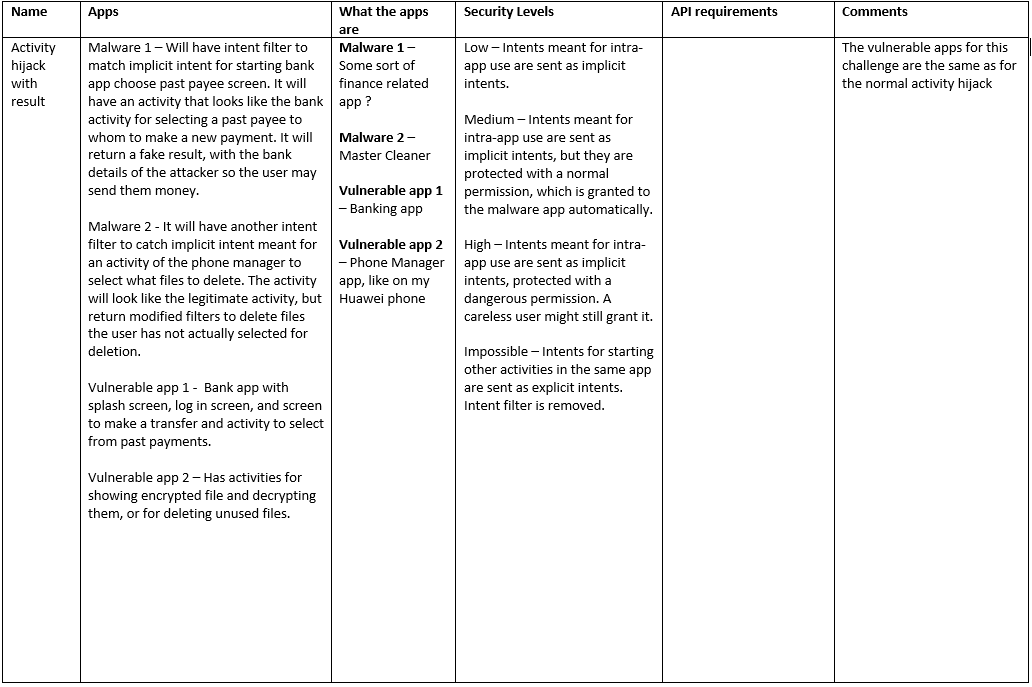
\includegraphics[width=1.4\textwidth]{graphics/activity_hijack_result_design.PNG}
        \caption{Preliminary design for Activity Intent Hijack with result challenge.}
        \label{fig:activity_hijack_result_design}
    \end{figure}
    
    \begin{figure}[h]
        \centering
        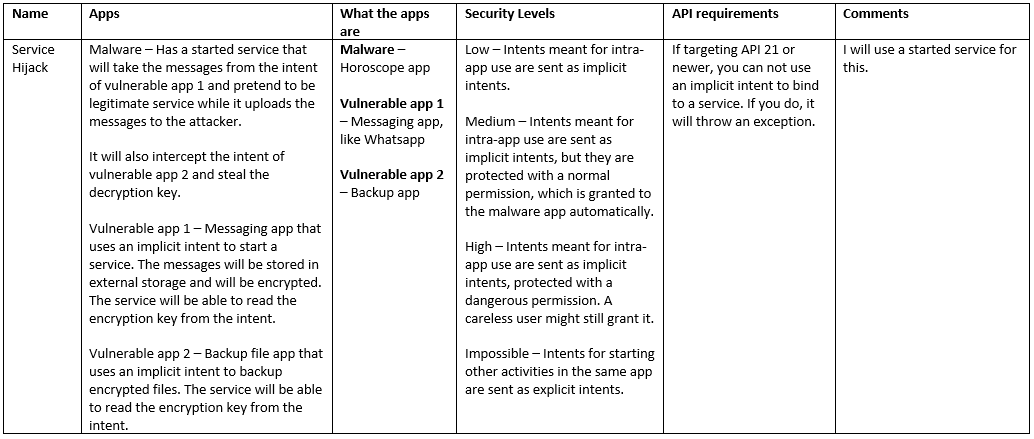
\includegraphics[width=1.4\textwidth]{graphics/service_hijack.PNG}
        \caption{Preliminary design for Service Intent Hijack challenge.}
        \label{fig:service_hijack_design}
    \end{figure}
    
    \begin{figure}[h]
        \centering
        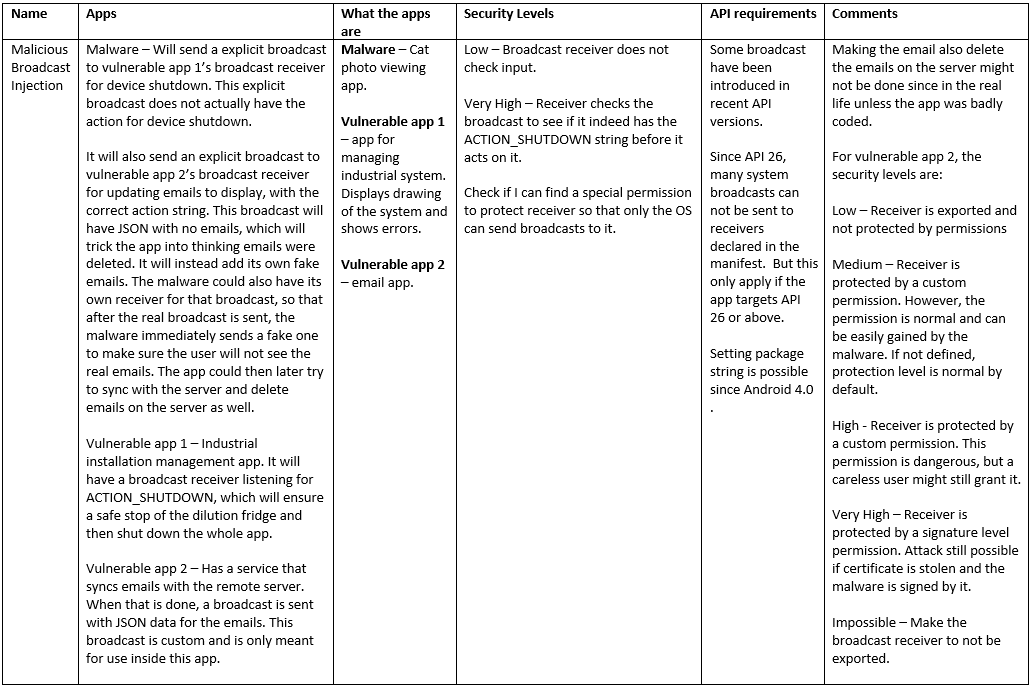
\includegraphics[width=1.4\textwidth]{graphics/malicious_broadcast_injection.PNG}
        \caption{Preliminary design for Malicious Broadcast Injection challenge.}
        \label{fig:malicious_broadcast_injection_design}
    \end{figure}
    
    \begin{figure}[h]
        \centering
        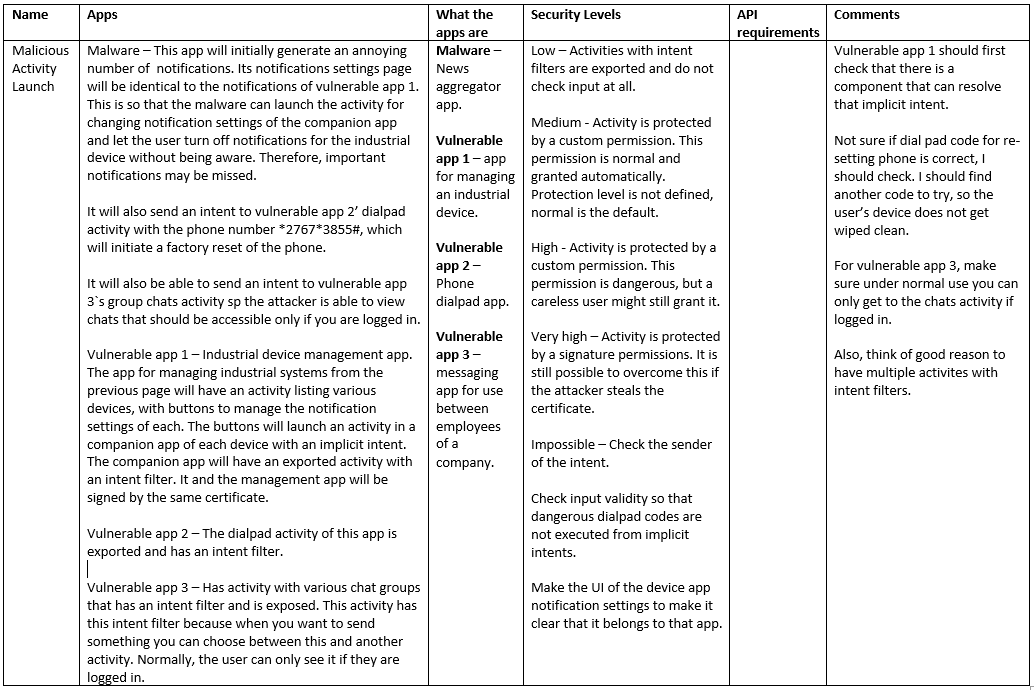
\includegraphics[width=1.4\textwidth]{graphics/malicious_activity_launch.PNG}
        \caption{Preliminary design for Malicious Activity Launch challenge.}
        \label{fig:malicious_activity_launch_design}
    \end{figure}
    
    \begin{figure}[h]
        \centering
        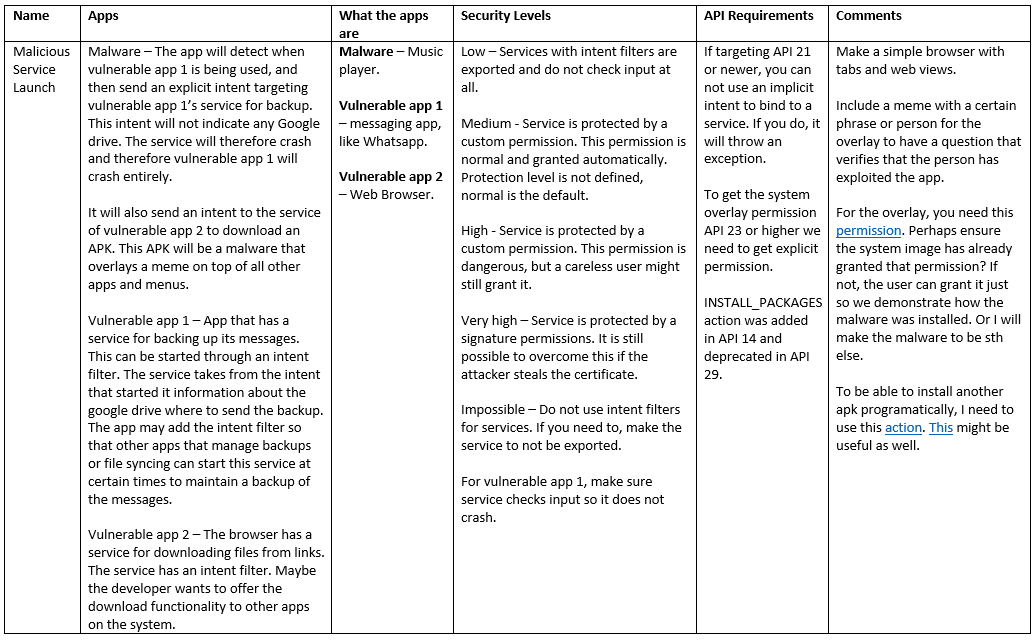
\includegraphics[width=1.4\textwidth]{graphics/malicious_service_launch.PNG}
        \caption{Preliminary design for Malicious Service Launch challenge.}
        \label{fig:malicious_service_launch_design}
    \end{figure}
    
    \begin{figure}[h]
        \centering
        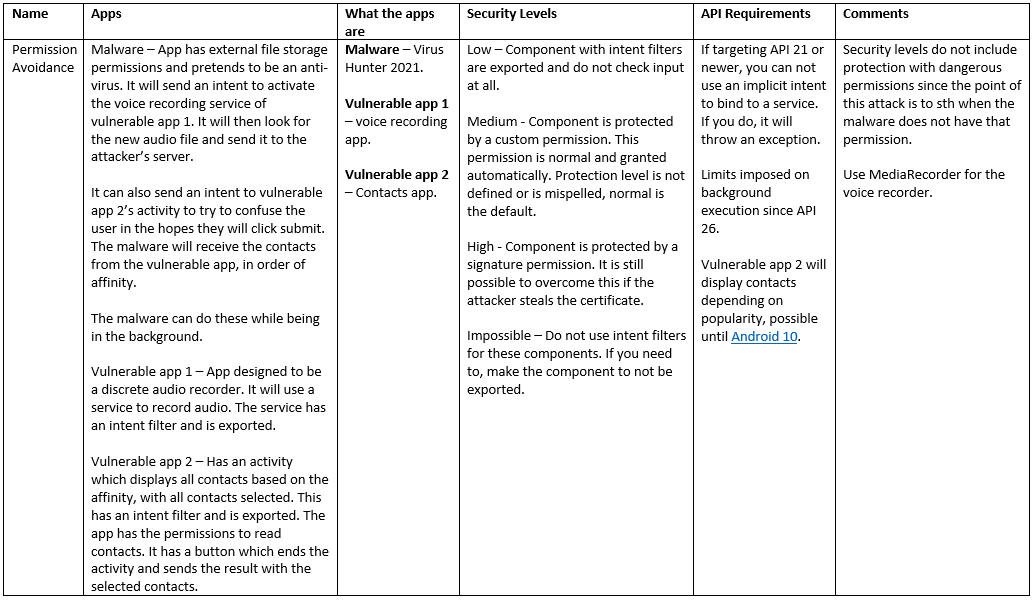
\includegraphics[width=1.4\textwidth]{graphics/permission_avoidance.PNG}
        \caption{Preliminary design for Permission Avoidance challenge.}
        \label{fig:permission_avoidance_design}
    \end{figure}
    
    \begin{figure}[h]
        \centering
        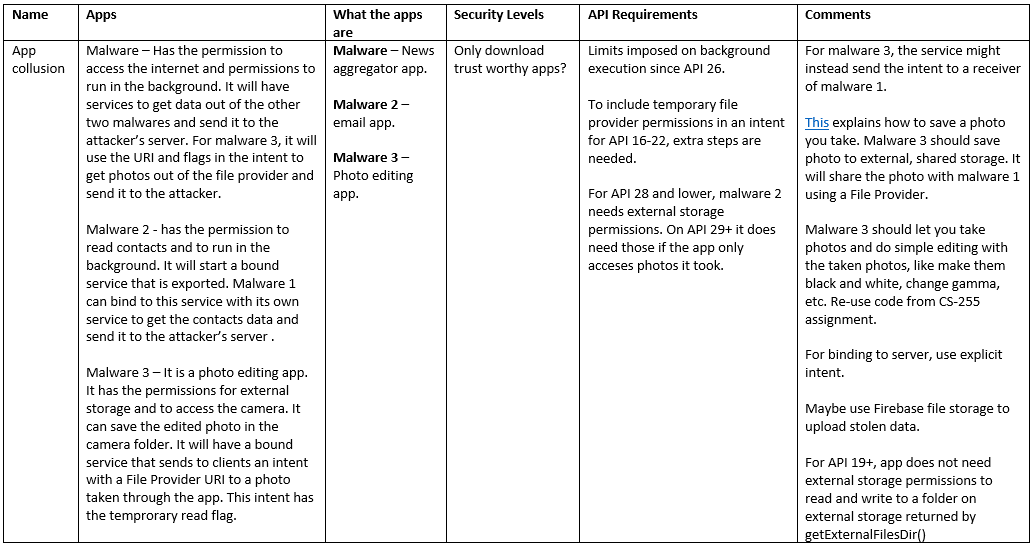
\includegraphics[width=1.4\textwidth]{graphics/app_collusion.PNG}
        \caption{Preliminary design for App Collusion challenge.}
        \label{fig:app_collusion_design}
    \end{figure}
\end{landscape}
